\section{Analytical Extrapolation}
\label{sec:analysis}
The capacity formulas of Section~\ref{sec:bounds} reproduce the simulated plateaus to within 3\% in every configuration we ran. That accuracy makes it reasonable to use them for questions that the simulator was not asked. Everything in this section is computed from the equations with the default parameters of Table~\ref{tab:params}. \emph{None of it was simulated}, so it is a prediction of the model and not a measurement. For the busy-wait policy we now also apply the link bound of Equation~\eqref{eq:llink}, which never binds at the default settings but does when more workers are added. The yield bound is $\Lambda_y$ as defined earlier.

\subsection{How many workers does each policy need?}
Solving the capacity equations for $N$ gives the number of workers that a policy needs to carry a load $\Lambda$ when the network is not the limit:
\begin{equation}
N_{bw}(\Lambda)=\Lambda\,S_{bw},\qquad N_{y}(\Lambda)=\Lambda\bigl(h\,t_L+(1-h)(t_c+2t_s)\bigr).
\label{eq:needed}
\end{equation}
Table~\ref{tab:workers} evaluates the two expressions. To carry 2.5~MRPS, the ceiling of the yield system, a spinning system would need 11.0 workers while a yielding system needs 5.1, which is a ratio of 2.2. Put differently, the eight workers of the simulated node are about 64\% busy at the yield ceiling, so the remaining capacity could be given to other tasks or to a smaller machine. We stress that these are capacity figures. A real system has to run below 100\% utilization to keep its tail latency bounded, as Figure~\ref{fig:p999} shows, so a deployment would add some margin to every entry.

\begin{table}[t]
\caption{Workers needed to carry a load, from Equation~\eqref{eq:needed} (derived, not simulated).}
\label{tab:workers}
\centering
\footnotesize
\begin{tabular}{rrr}
\toprule
Load (MRPS) & Busy-wait & Yield \\
\midrule
1.5 & 6.6 & 3.1 \\
2.0 & 8.8 & 4.1 \\
2.5 & 11.0 & 5.1 \\
\bottomrule
\end{tabular}
\end{table}

Figure~\ref{fig:scale}(a) illustrates how saturation scales with core count. The yield curve climbs steeply with $N$ until hitting the network bottleneck at $N \approx 5.1$ workers, plateauing thereafter because the 100~GbE link cannot serialize more pages. The busy-wait curve scales with core count more gradually, taking $N \approx 11$ workers to reach that same link ceiling. This reveals a critical architectural insight: yielding provides the biggest efficiency dividend when CPU cores are scarce relative to link bandwidth. At 4 cores, yielding offers $2.16\times$ higher capacity; at 8 cores, $1.38\times$; and beyond 11 cores, both policies saturate the physical link equally. Adios evaluated only $N=8$, so this scaling cross-over is an original prediction of our model.

\subsection{Sensitivity to the fetch time}
The busy-wait capacity depends on the fetch time because a spinning worker is occupied for all of it, whereas the yield capacity at the link limit does not. Figure~\ref{fig:scale}(b) varies the unloaded fetch time $t_f$ from 2 to 6~$\mu$s with every other parameter fixed. The predicted capacity ratio is 1.13 at 2~$\mu$s, 1.38 at the default 3~$\mu$s, 1.63 at 4~$\mu$s, 1.88 at 5~$\mu$s and 2.13 at 6~$\mu$s. The break-even switch cost of Equation~\eqref{eq:breakeven} rises in step, from 1.0 to 3.0~$\mu$s. Both trends say the same thing: the slower the remote memory, the more there is to gain by hiding it. The lower end of the range (2--3~$\mu$s) is the one reported for a 4~KiB read on a 100~GbE card \cite{adios}. Larger values would correspond to a more distant memory node, a congested fabric or a slower technology, and the model suggests that yielding becomes more attractive in each of those cases. This reading agrees with the motivation of the original paper, although neither it nor our simulator tests it directly.

\begin{figure*}[t]
\centering
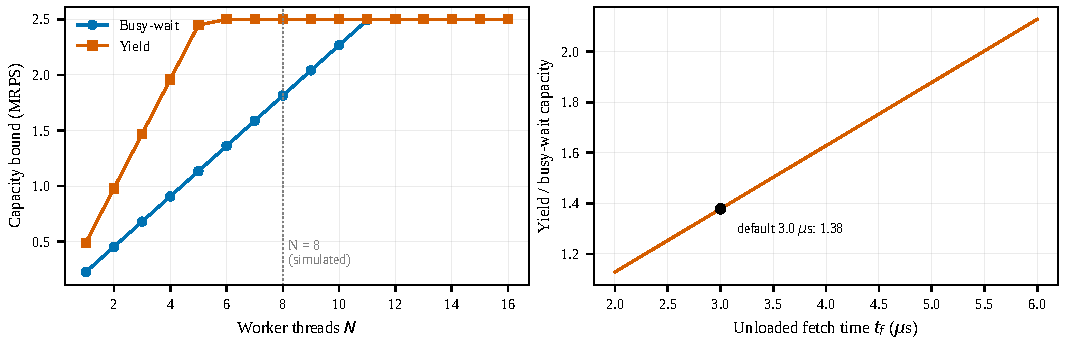
\includegraphics[width=0.92\textwidth]{scale}
\caption{Analytical predictions (not simulated). (a) Capacity bound against the number of workers for $h=20\%$. (b) Ratio of the yield capacity to the busy-wait capacity against the unloaded fetch time, for $N=8$.}
\label{fig:scale}
\end{figure*}

\subsection{Concurrency of fetches}
Little's law relates the average number of fetches in flight to the completion rate and the time each fetch takes. At the plateau of the busy-wait system, 1.77~MRPS with 80\% of requests missing and a fetch of at least 3.0~$\mu$s, there are on average at least $1.77\times0.8\times3.0\approx4.2$ fetches outstanding, out of at most eight. The yield system at 2.50~MRPS carries at least $2.50\times0.8\times3.0=6.0$, which is 0.75 per queue pair. Because queueing at the link lengthens each fetch beyond its unloaded time, both figures are lower bounds. They show that the spinning system leaves almost half of its possible fetch slots empty on average, and that the yield system uses more of them with the same number of workers. This is the quantitative form of the under-utilization argument that Section~\ref{sec:background} gave in words, and it again agrees with the direction reported for the real system, where the link utilization rises from about 50\% to 82\% \cite{adios}.

\subsection{Summary of the Predictions}
In summary, our analytical model yields three concrete takeaways:
\begin{enumerate}
\item \emph{Hardware footprint}: Yielding achieves target throughput with under half the physical cores required by busy-waiting under default parameters (5.1 vs.\ 11.0 workers for 2.5~MRPS).
\item \emph{Sensitivity to network delay}: Slower remote fetch times widen yielding's throughput advantage over spinning, making yielding increasingly attractive on congested or multi-hop networks.
\item \emph{Break-even threshold}: Yielding's throughput advantage disappears whenever thread context switching exceeds $t_f / 2 = 1.5~\mu$s, explaining why kernel-level paging must spin while unikernel unithreads can yield.
\end{enumerate}
